\section{H Scintillator}
Since the time resolution is proportional to $\sqrt{N_{pe}}$, in order to improve the time resolution, the scintillator material for the TOF system must have fast decay times, long attenuation length, and good spectral match to the PMTs. The attenuation length of scintillator can be divided into two parts. One part is called the technical attenuation length (TAL), which is defined as the length reducing the amount light by a factor e and which depends
on the geometry the scintillator and the reflective properties of its surface. The other part is called bulk attenuation length (BAL), which reduces the initial light intensity by a factor $e$ according to the Buger-Lambert Law and which depends on the transparency and the scintillation material. From the design requirement, the counter length of CLAS12 panel 1b detectors varies from $17.27cm$ to $407.9cm$, so it is important to find the right material for all counters. The Table~\ref{table1} shows that scintillator material $EJ200$ and $BC408$ both have longer attenuation length and slower decay time. $EJ204$ and $BC404$ both have shorter attenuation length and faster decay time. The time resolution of these scintillator material for $50$ $cm$-long bars are measured. The comparison results are shown in Fig.~\ref{f:TRmaterial}, there is no big difference between different material.

\begin{table}[h]
\begin{center}
\begin{tabular}{|c|c|}
\hline
Plastic Scintillator &
\multicolumn{1}{|c|}{Decay Time}\\
\hline
EJ200  &     2.1ns (slow)\\
EJ204  &     1.8ns (fast)\\
BC408  &     2.1ns (slow)\\
BC404  &     1.8ns (fast)\\
\hline
\end{tabular}
\caption{Scintillator comparing}
\label{table1}
\end{center}
\end{table}

The parametrization of $\overline{\sigma_{ToF}}$ is used to study the possible improvements in time resolution based on a trade-off between the decay time of the scintillator and the number of photoelectrons arriving at the PMT, which depends on the attenuation length~\cite{smith1999time}. Fig.~\ref{f:tradeoff} shows the expected time resolution plotted as a function. Based on the fast decay time of $BC404$, it is used as shorter bar's material. For longer counters, the existing material $BC408$ with its larger attenuation length is the better choice. In the Fig.~\ref{f:tradeoff} there is a time resolution crossing point around $200$ $cm$. Below it, the counters with $BC404$ material have better time resolution and above it, the $BC408$ counters have better time resolution. From the above information, we decided to use $BC404$ material for the length of counters shorter than $200$ $cm$ and $BC408$ material for the counters longer than $200$ $cm$.

\begin{figure}
\centerline{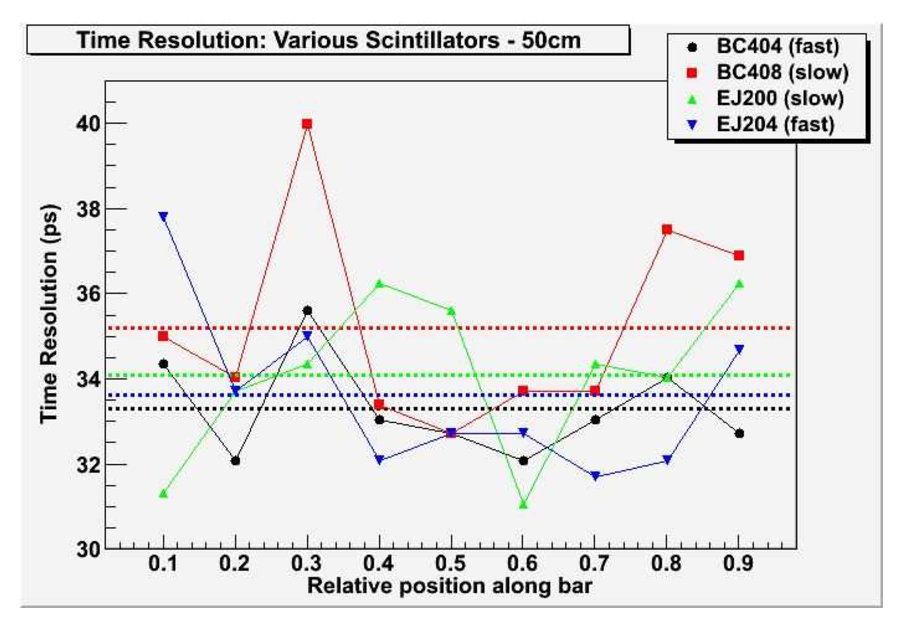
\includegraphics[width=13cm,height=10cm]{ye/fig_ye_scintillator/s0.pdf}}
\caption{The time resolution of different scintillator material (50cm scintillator bars )}
\label{f:TRmaterial}
\end{figure}

Initial measurements show that attenuation length values vary even among scintillation
bars of the same material and from the same mold, so in order to verify that
each counter meets required specifications, the attenuation length measurement is
incorporated into the unit testing of each counter constructed for Panel 1B. There are two methods used to measure the attenuation length. One is the cosmic ray method, which we use the same data collected in the three-bar time resolution measurements, described in Sec.III B. Figure~\ref{f:ADC} shows the Offset-corrected ADC values, which are directly proportional to the number of photons arriving at the photocathode are plotted against TDC difference values $(\frac{TDC_{L}-TDC_{R}}{2})(also called \Delta t)$ , which are proportional to the position through which the ionizing particles pass. To find the maximally occurring ADC value for each $\Delta t$ slice, ADC distributions for each TDC difference interval are fit with Gauss-convoluted Landau functions. The ADC provides a measure of the number of photons reaching the photocathode, and the left and right TDCs provide the time information needed to reconstruct the impact position based on the effective speed of light in the scintillator. The attenuation length parameters, TAL and BAL, of the scintillator are given by,
\begin{equation}
N=N_{0T}e^{-\frac{x}{\lambda_{T}}}+N_{0B}e^{-\frac{x}{\lambda_{B}}}
\label{eq:2}
\end{equation}
where $N_{0} = N_{0T} + N_{0B}$ is the initial number of photons caused by the cosmic ray passing
through the scintillator at the impact position $x$ and $N$ is the number of photons arriving
at the PMT. Figure~\ref{f:ADCTDC} illustrates the relationship between $N$ (ADC) and $x((TDC_{L}-TDC_{R})/2)$
for the data. Slices of the TDC difference values are projected onto the ADC axis, and fit
with Gauss-convoluted Landau functions from which the most probable ADC value for each
position is obtained (Fig.~\ref{f:ADC}). These new pairs of data points are fit by various ans\"{a}tze
of exponential functions to extract the attenuation length parameters, as shown in Fig.~\ref{f:expo}.
\begin{figure}[h!]
\begin{minipage}[h]{0.5\linewidth}
\centering
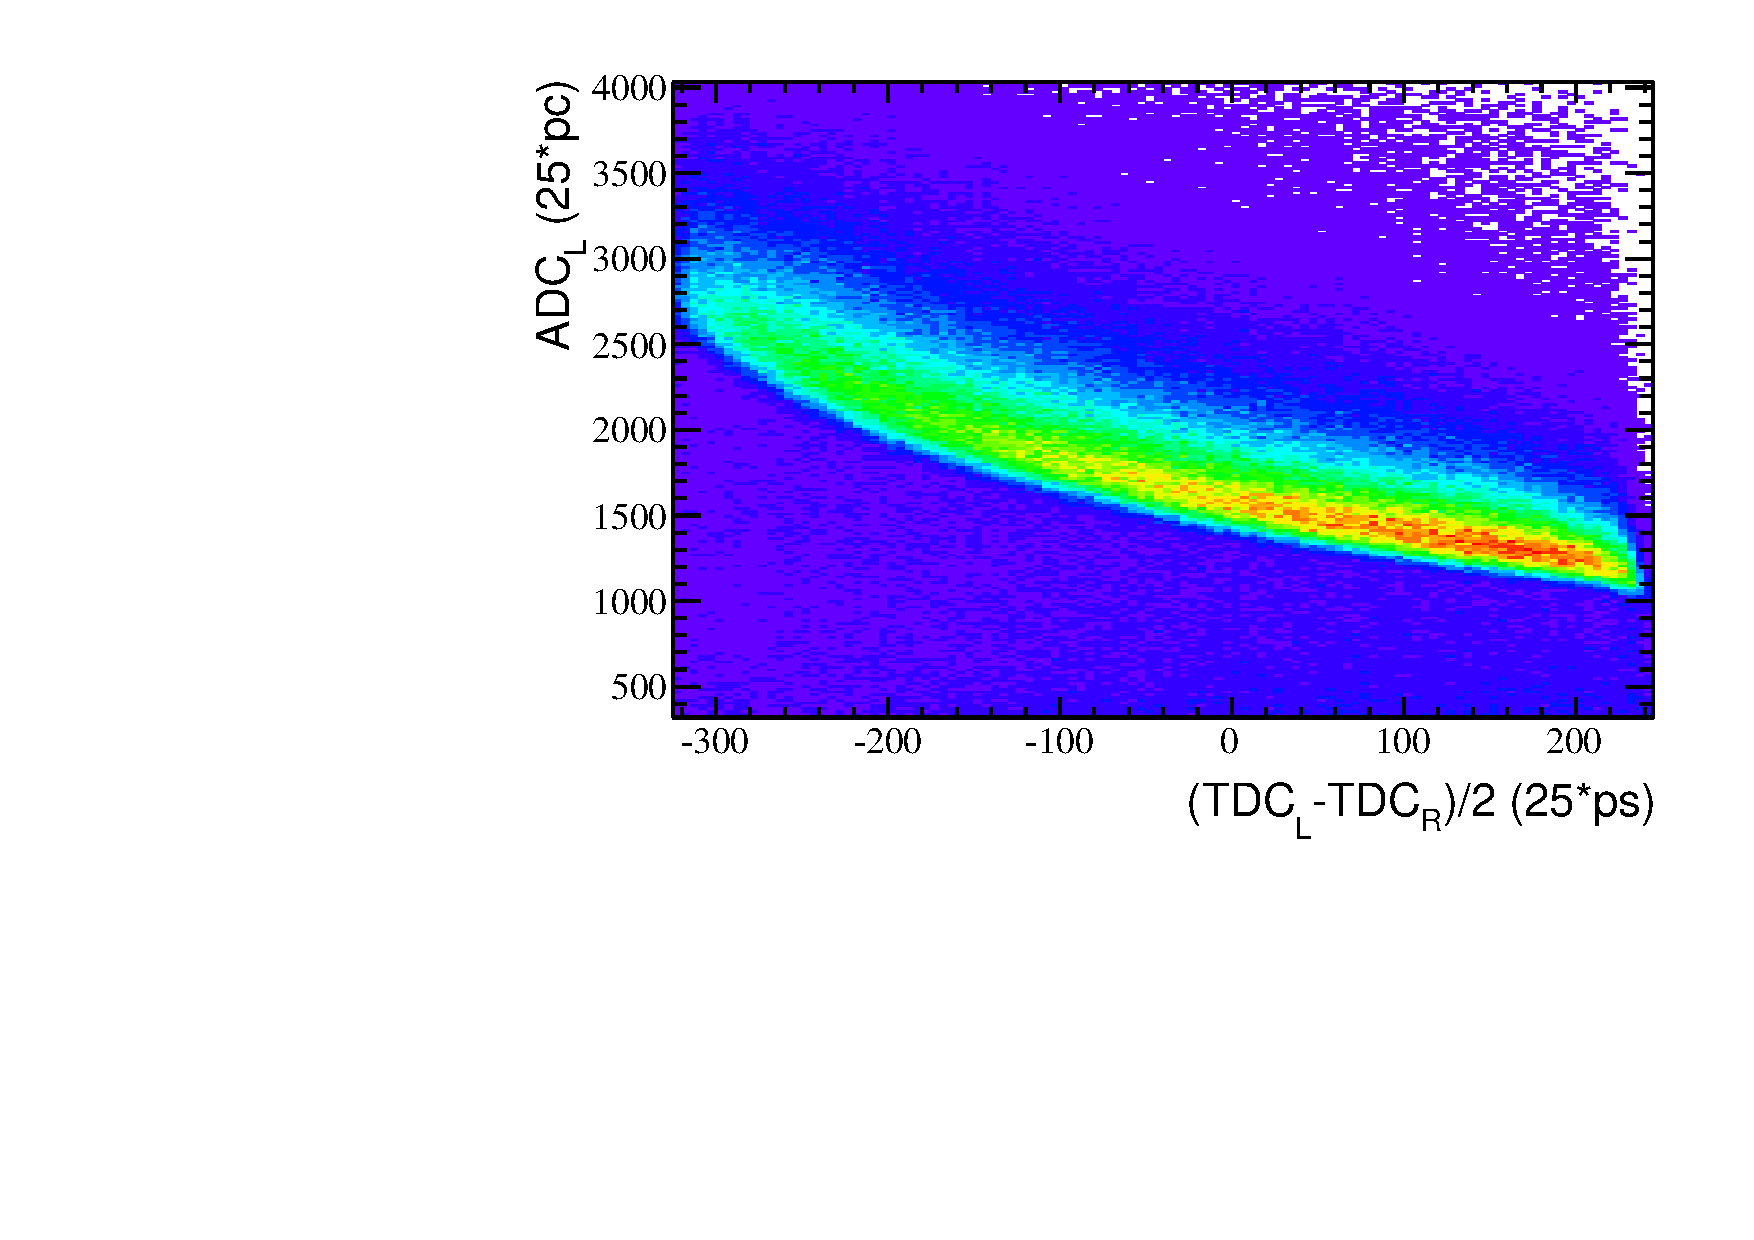
\includegraphics[width=2.5in]{ye/fig_ye_scintillator/c2_L.pdf}
\end{minipage}%
\begin{minipage}[h]{0.5\linewidth}
\centering
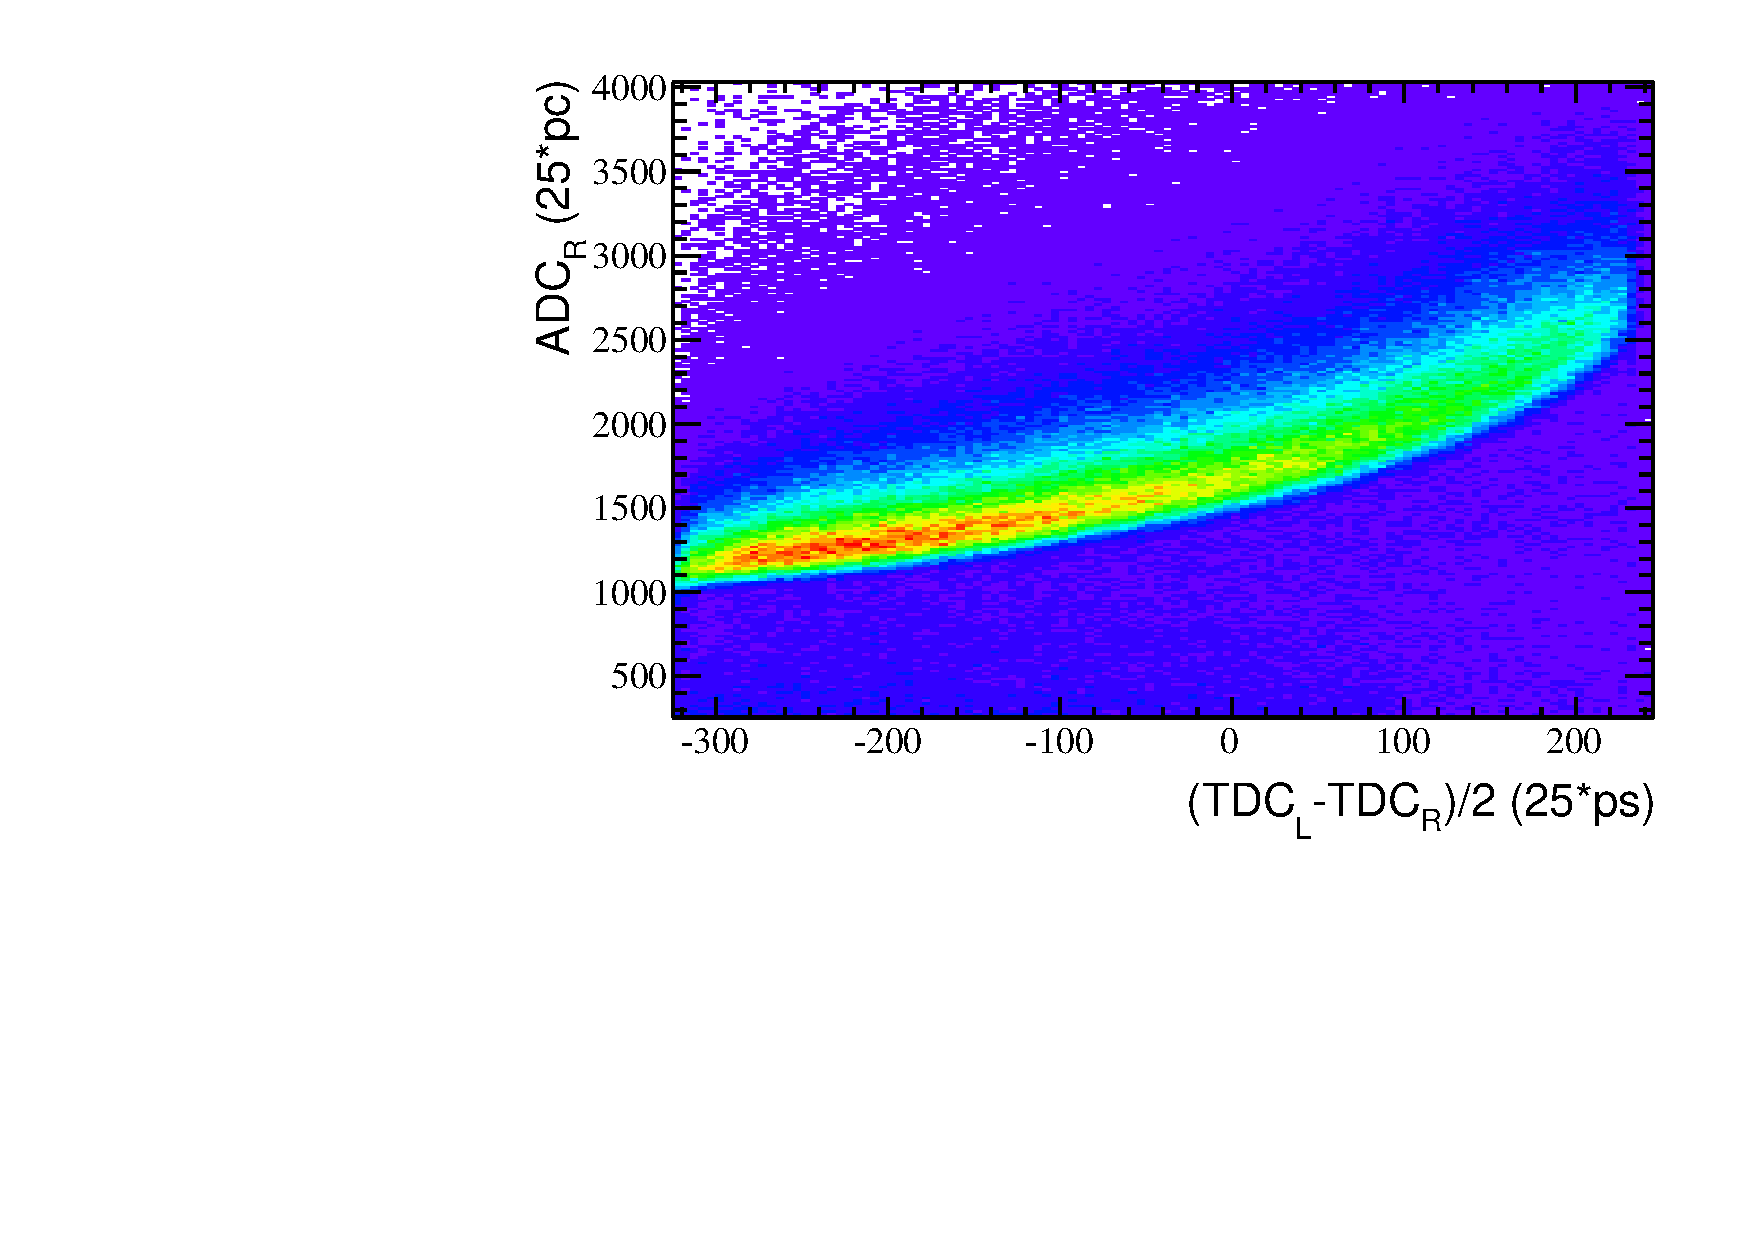
\includegraphics[width=2.5in]{ye/fig_ye_scintillator/c2_R.pdf}
\end{minipage}
\caption{Left and right $ADC_{L}$ and $ADC_{R}$ versus TDC difference for a $6cm\times6cm\times210cm$ bar}
\label{f:ADCTDC}
\end{figure}


And the other is the ource method, the $Sr-90$ source was put on the top of one scintillator at $5cm$ away from left side, then use the same electronic setups as three bar method. After the data satisfy the statistic requirement, move the source to the position of $15$cm away from left side of the bar and repeat the same step. For the position part, there is $10$cm away between each measurement position point. After the measurement, the data analysis steps are similar with the cosmic ray method, the only different is the ADC value which is subtracted by the cosmic ray signal background. After subtracting, fit the mean value of the ADC distribution of the fixed position versus the position distribution by the exponential function~\ref{eq:2} to get the TAL and BAL attenuation length, which shows in Fig.6. Here, it is a approvement that the attenuation length have two components, can not be fit well by the single exponential function.

\begin{figure}[ht!]
\centerline{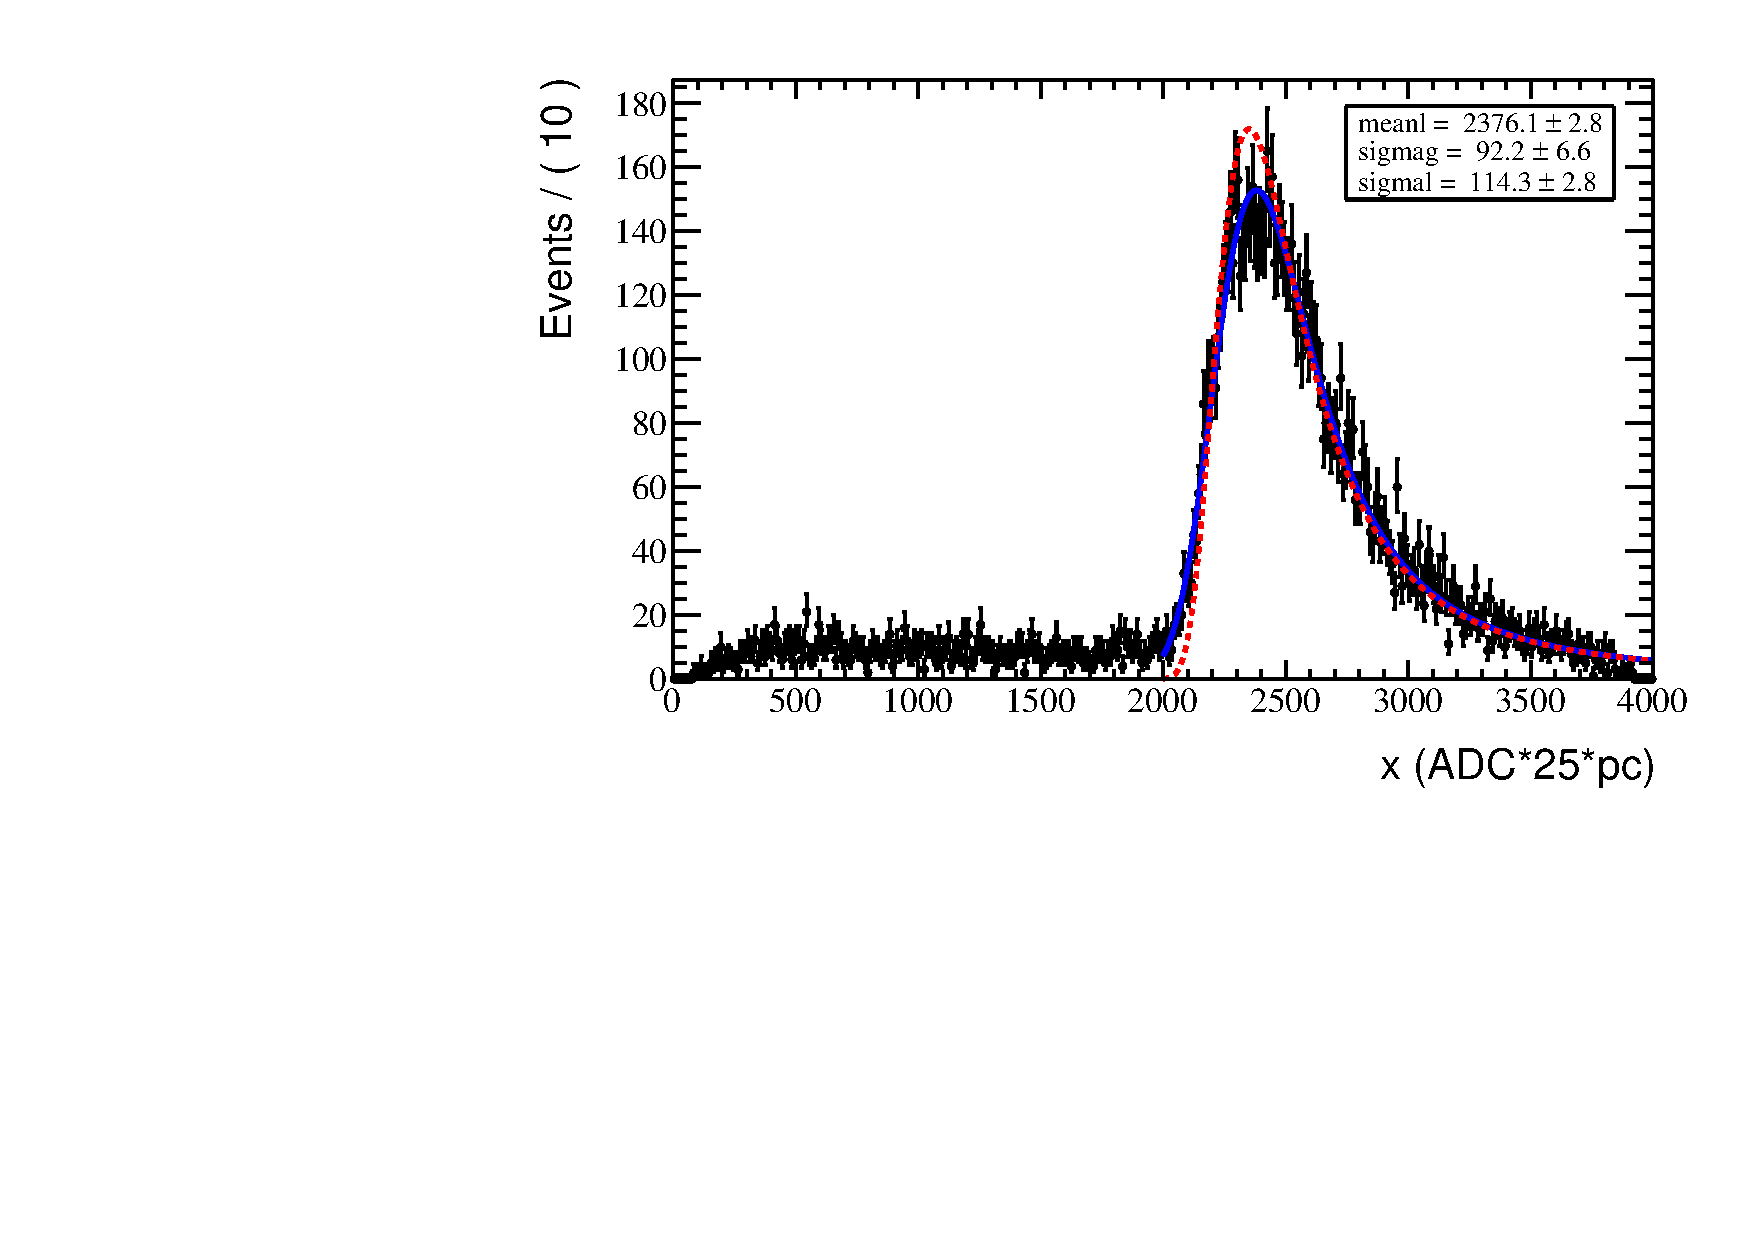
\includegraphics[width=13cm,height=10cm]{ye/fig_ye_scintillator/ADC.pdf}}
\caption{Gauss-convoluted Landau fit of the ADC distribution for a central single TDC difference
slice for the BC-408 210 cm-long bar, where x represents the ADC value, and "Maximum
x" is hence the most probable ADC value. The blue line shows Gauss-convoluted Landau fit, the red dashed line shows Landau fit only.
 }
\label{f:ADC}
\end{figure}


\begin{figure}[h!]
\begin{minipage}[h]{0.5\linewidth}
\centering
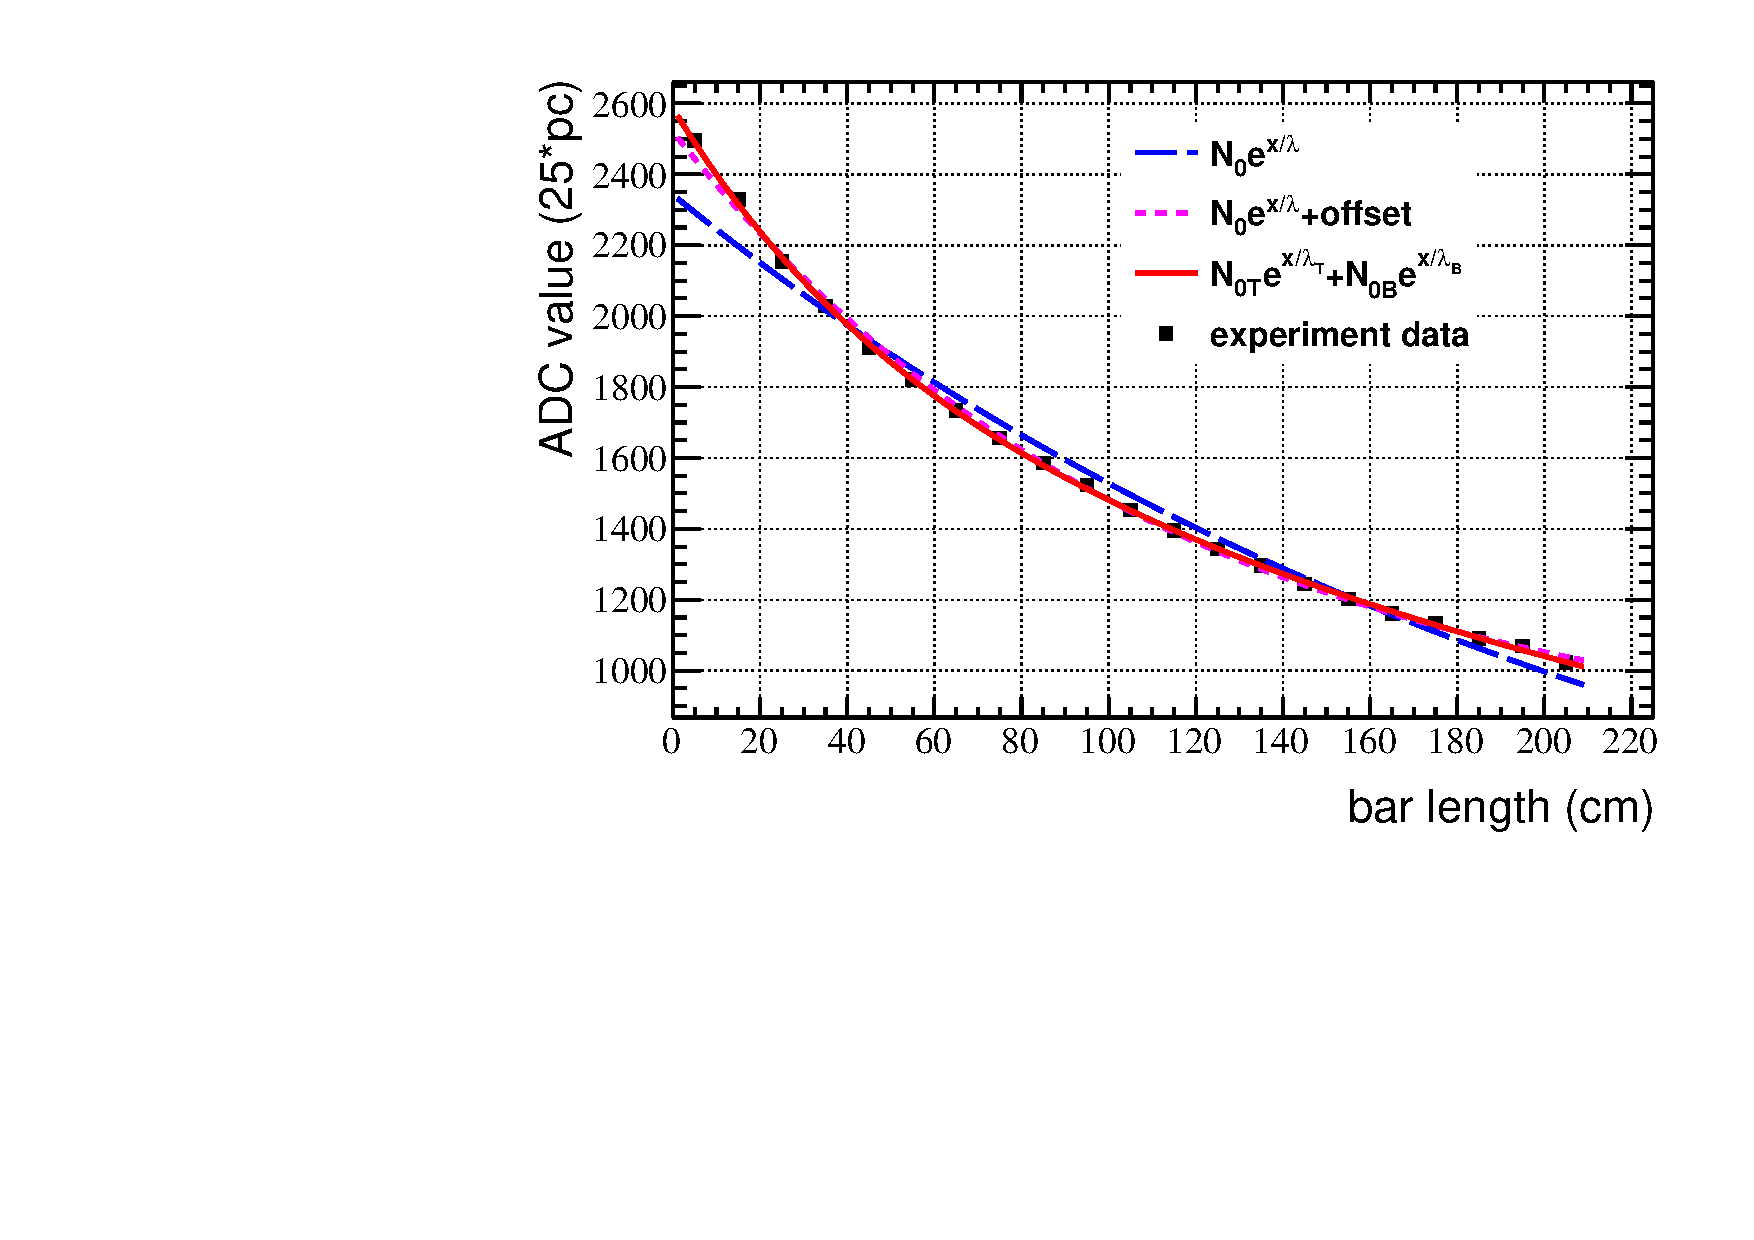
\includegraphics[width=3in]{ye/fig_ye_scintillator/c1_TL.pdf}
\end{minipage}%
\begin{minipage}[h]{0.5\linewidth}
\centering
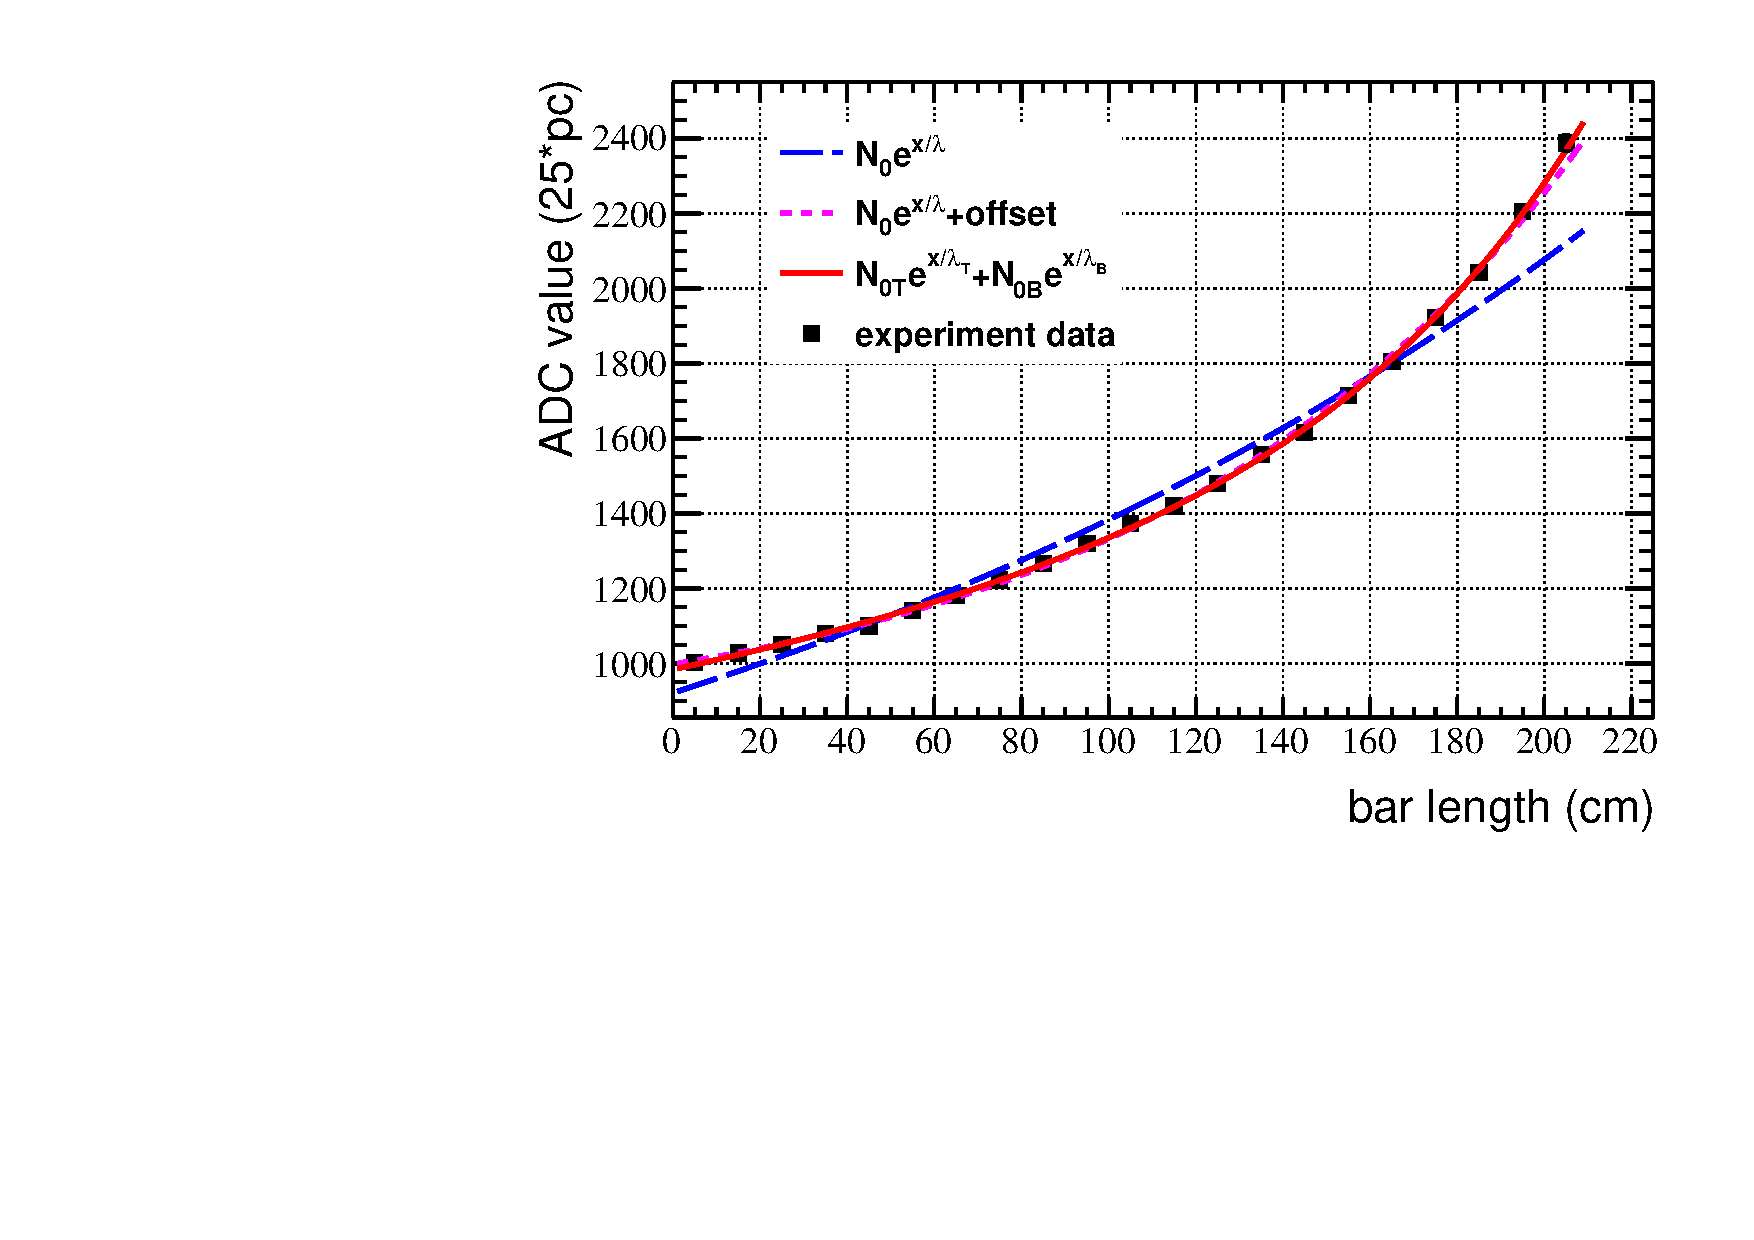
\includegraphics[width=3in]{ye/fig_ye_scintillator/c1_TR.pdf}
\end{minipage}

\caption{ADC versus TDC difference for the left and right PMTs of the $BC408$ $210 cm$-long bar. The black square shows most probable ADC value points corresponding to the bar length , the red line shows two exponential function fit, the blue long dashed line shows on exponential fit, the magenta short dashed line shows one exponential function with offset fit.}
\label{f:expo}
\end{figure}


Finally, in order to compare with the factory attenuation length value, we use two points method to get the attenuation length (same method as factory used to get their attenuation length value using laser system?). The two positions($15cm$ and $195cm$ away form the left side of the bar) are chosen to get the ADC values, and then fit this two data points by one exponential function to get the corresponding attenuation length. The comparison results are shown on Table~\ref{table2} and Table~\ref{table3}. we got consistent attenuation length value less than the factory value with both cosmic ray and source measurements, but for the first order acceptable. This is one of the quality check procedure.
\newpage
\begin{landscape}
\begin{table}[htbp]
\centering
\caption{Attenuation Length (AL) Table ($210$ cm bar) Source Method}
\begin{tabular}{|c|c|c|c|c|c|c|c|}
\hline
\multirow{2}{*}{Scintillator}
& \multirow{2}{*}{PMT}
& \multirow{2}{*}{2 points AL (cm)}
& \multirow{2}{*}{2 points AL (cm)}
& \multirow{2}{*}{2 points AL (cm)}
& \multirow{2}{*}{2 points AL (cm)}
& \multicolumn{2}{|c|}{21 points AL (cm)}\\
\cline{7-8}
type & Position & (15 and 195 cm) & (25 and 185 cm) & (35 and 175 cm) & (45 and 165 cm) & BAL & TAL \\
\hline
\multirow{2}{*}{LAL Factory AL}
& Left
& 178.09 $\pm$ 0.27
& 181.96 $\pm$ 0.34
& 185.98 $\pm$ 0.39
& 188.24 $\pm$ 0.46
& 250.03 $\pm$ 1.37
& 43.34 $\pm$ 0.47 \\
\cline{2-8}
(280cm) & Right & 238.06 $\pm$ 0.50 & 252.89 $\pm$ 0.63 & 261.51 $\pm$ 0.77
& 276.94 $\pm$ 1.00 & 332.33 $\pm$ 0.89 & 26.59 $\pm$ 0.20 \\
\hline
\end{tabular}
\label{table2}
\end{table}


\begin{table}[htbp]
\centering
\caption{Cosmic Ray Method}
\begin{tabular}{|c|c|c|c|c|c|c|c|}
\hline
\multirow{2}{*}{Scintillator}
& \multirow{2}{*}{PMT}
& \multirow{2}{*}{2 points AL (cm)}
& \multirow{2}{*}{2 points AL (cm)}
& \multirow{2}{*}{2 points AL (cm)}
& \multirow{2}{*}{2 points AL (cm)}
& \multicolumn{2}{|c|}{21 points AL (cm)}\\
\cline{7-8}
type & Position & (15 and 195 cm) & (25 and 185 cm) & (35 and 175 cm) & (45 and 165 cm) & BAL & TAL \\
\hline
\multirow{2}{*}{LAL Factory AL}
& Left
& 231.31 $\pm$ 8.09
& 234.95 $\pm$ 7.78
& 240.84 $\pm$ 9.51
& 241.45 $\pm$ 11.89
& 330.6 $\pm$ 43.1
& 48.3 $\pm$ 12.7 \\
\cline{2-8}
(280cm) & Right & 235.85 $\pm$ 8.61 & 240.33 $\pm$ 10.82 & 242.51 $\pm$ 11.00
& 241.97 $\pm$ 11.73 & 462.0 $\pm$ 167.1 & 58.8 $\pm$ 18.1 \\
\hline
\end{tabular}
\label{table3}
\end{table}

*AL---Attenuation Length                    *LAL---Long Attenuation Length
*2 points---1 exponential function method   *BAL---Bulk Attenuation Length
\end{landscape}
\newpage


\begin{figure}[ht!]
\centerline{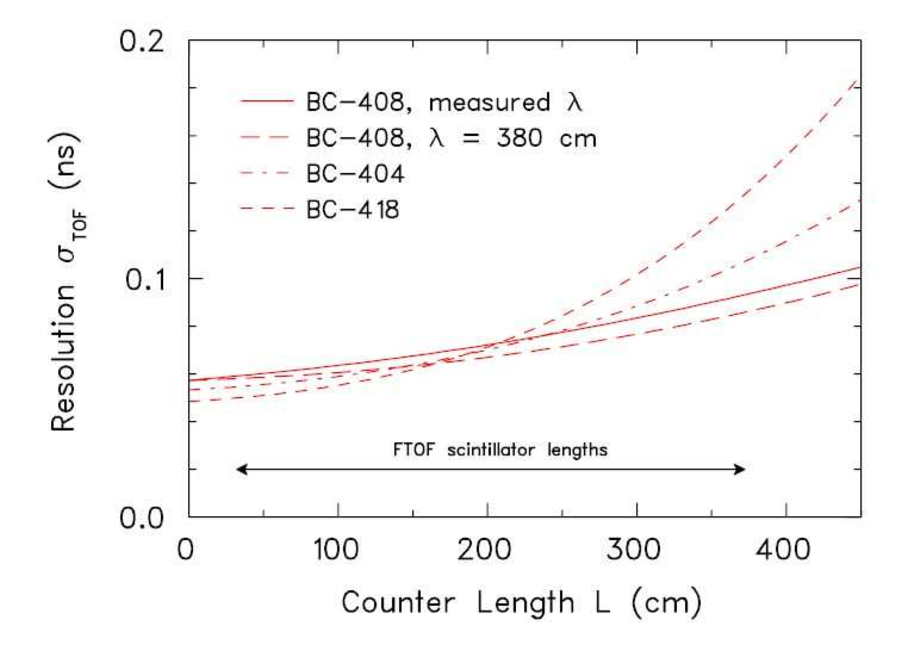
\includegraphics[width=13cm,height=10cm]{ye/fig_ye_scintillator/S2.pdf}}
\caption{Resolution for various scintillation materials showing the trad-off between attenuation length and decay time ~\cite{clasclas12}}
\label{f:tradeoff}
\end{figure}
